\documentclass[12pt,a4paper,oneside]{article}

\usepackage[utf8]{inputenc}
\usepackage{enumitem}

\newenvironment{uc}[1]{
    \vspace{10pt}
    \textbf{Use Case: #1}
    \setlength{\parskip}{0pt}
    \setlength{\parindent}{0pt}
}{
    \vspace{10pt}
}

\newcommand{\ucpart}[1]{\vspace{5pt}{\bfseries #1}\vspace{5pt}}
\newcommand{\extends}[1]{Extends: \emph{#1}}
\newcommand{\extend}[1]{$<<$Extend #1$>>$} 
\newcommand{\return}[1]{\item Return to MSS step #1.}

\newenvironment{uc-ol}[1]{
    \begin{enumerate}[itemsep=0pt,topsep=0pt,leftmargin=*,labelindent=#1]
    \linespread{1}
}{
    \end{enumerate}
}

\newenvironment{uc-ul}[0]{
    \begin{itemize}[topsep=0pt,itemsep=0pt]
    \setlength{\itemindent}{10pt}
}{
    \setlength{\itemindent}{0pt}
    \end{itemize}
}

\newenvironment{uc-mss}[1]{
    \ucpart{Main Success Scenario: #1}
    \begin{uc-ol}{10pt}
}{
    \end{uc-ol}
}

\newenvironment{uc-ext}[0]{
    \ucpart{Extensions}
}{ }

\newenvironment{uc-fail}[2]{
    \vspace{5pt}
    \let\itemb\item
    \renewcommand\item{\stepcounter{enumi}\itemb[#1$.$\theenumi$:$]}
    \hspace{20pt} \textbf{$<$MSS STEP #1$>$  [#2]}
    \begin{uc-ol}{30pt}
}{
    \end{uc-ol}
    \vspace{10pt}
}

\newenvironment{uc-pre}[0]{
    \ucpart{Pre-conditions:}
    \begin{uc-ul}
}{
    \end{uc-ul}
}
  
\newenvironment{uc-post}[0]{
    \ucpart{Post-conditions:}
    \begin{uc-ul}
}{
    \end{uc-ul}
}

\newenvironment{uc-trig}[0]{
    \ucpart{Triggers:}
     \begin{uc-ul}
}{
	\end{uc-ul}
}

 \linespread{1.3}
 
\usepackage{longtable}
\usepackage[dutch]{babel}
\usepackage{titling,enumitem}
\usepackage{graphicx}
\usepackage{tikz}
\usepackage{a4wide}
\usepackage{amsmath}
\usepackage{amssymb}
\usepackage{rotating}
\usepackage{listings}
\usepackage{float}
\usepackage{color}
\usepackage{fancyhdr}
\usepackage{lastpage}
% packages
\usepackage[T1]{fontenc}
\usepackage[margin=3cm]{geometry}
\usepackage{array, xcolor}
\usepackage{titling}
\usepackage{blindtext}
\usepackage{pdfpages}
% rules
\definecolor{lightgray}{gray}{0.8}
\newcolumntype{L}{>{\raggedleft}p{0.50\textwidth}}
\newcolumntype{R}{p{0.8\textwidth}}
\newcommand\VRule{\color{lightgray}\vrule width 0.5pt}
\renewcommand{\footrulewidth}{0.4pt}% default is 0pt
\renewcommand \thesection{\Roman{section}}
\renewcommand \thesubsection{\arabic{subsection}}
\setlength\parindent{0pt}
%%%%%%%%%%%%TABULAR SHIT%%%%%%%%%%%%%%%%%%
\usepackage{color, colortbl}
\definecolor{Gray}{gray}{0.9}
%%%%%%%%%%%%%%%%%%%%%%%%%%%%%%%%%%%%%%%%
%SECTION SHIT
\renewcommand*{\thesubsubsection}{\Alph{section}}
\definecolor{dkgreen}{rgb}{0,0.6,0}
\definecolor{gray}{rgb}{0.5,0.5,0.5}
\definecolor{mauve}{rgb}{0.58,0,0.82}
 
\lstset{ %
  language=Java,                
  basicstyle=\footnotesize,           
  numbers=left,                  
  numberstyle=\tiny\color{gray},  
  stepnumber=2,                        
  numbersep=5pt,                  
  backgroundcolor=\color{white},      
  showspaces=false,               
  showstringspaces=false,        
  showtabs=false,                 
  frame=single,                   
  rulecolor=\color{black},        
  tabsize=2,                      
  captionpos=b,                   
  breaklines=true,                
  breakatwhitespace=false,        
  title=\lstname,                                                  
  keywordstyle=\color{blue},          
  commentstyle=\color{dkgreen},       
  stringstyle=\color{mauve},         
  escapeinside={\%*}{*)},            
  morekeywords={*,...},              
  deletekeywords={...}              
}
\begin{document}

\includepdf[pages={1}]{titlepage.pdf}
\pagestyle{fancy}
\fancyhf{}
\fancyhead[R]{Groep 16}
\fancyhead[L]{SO2: Behoeftenanalyse en Architectuur}
\fancyfoot[L]{\small Vakgroep Informatietechnologie \\ Gaston Crommenlaan 8, bus 201, B - 9050 Gent \\ www.intec.UGent.be}
\fancyfoot[R]{\raisebox{3ex-\height}{\small \thepage / \pageref{LastPage} \,
\includegraphics{intec.png}}}
\noindent We kozen ervoor om de \textbf{Augmented Reality} applicatie verder uit te werken.
\section{Systeemontwerp}
\subsection{Subsystemen}
\subsubsection*{Analyse}
\begin{longtable}{|p{5cm}|p{11cm}|}
\hline\rowcolor{Gray}
\textbf{Relevante klassen} & \textbf{Verantwoordelijkheden}\\ 
\hline
FotoAnalyser&Neemt foto's en stuurt deze door naar de servercommunicatie. De informatie die hij terug krijgt wordt door gegeven aan de applicatie. \\
\hline
\end{longtable}

\subsubsection*{Camera}
\begin{longtable}{|p{5cm}|p{11cm}|}
\hline\rowcolor{Gray}
\textbf{Relevante klassen} & \textbf{Verantwoordelijkheden}\\ 
\hline
Camera&Het maken van de foto's.\\
\hline
Multimedia&Een foto/video en zijn eigenschappen.\\
\hline
\end{longtable}

\subsubsection*{Servercommunicatie}
\begin{longtable}{|p{5cm}|p{11cm}|}
\hline\rowcolor{Gray}
\textbf{Relevante klassen} & \textbf{Verantwoordelijkheden}\\ 
\hline
Connection&De connectie met de backend. Bevat methodes om data te ontvangen/te versturen.\\
\hline
Network&Maakt een nieuwe connectie aan. Bevat methodes voor het analyseren van foto's (wat op de server gebeurt) en het aanpassen/toevoegen van info in de databank.\\
\hline
ConnectionListener&Luistert naar binnenkomende Connections.\\
\hline
OverlayDataObject&Algemeen data-object dat kan weergegeven worden op de bril. Dit kan vergeleken worden met een HTML-pagina, die video's, foto's en tekst kan bevatten.\\
\hline
\end{longtable}

\subsubsection*{Leermodus}
\begin{longtable}{|p{5cm}|p{11cm}|}
\hline\rowcolor{Gray}
\textbf{Relevante klassen} & \textbf{Verantwoordelijkheden}\\ 
\hline
InformationEditor&Communicatieklasse met servercommunicatie, bevat de informatie die moet toegevoegd/aangepast worden.\\
\hline
\end{longtable}

\subsubsection*{Audio}
\begin{longtable}{|p{5cm}|p{11cm}|}
\hline\rowcolor{Gray}
\textbf{Relevante klassen} & \textbf{Verantwoordelijkheden}\\ 
\hline
AudioInput&Het commando van de gebruiker.\\
\hline
VoiceCommandRecognizer&Zorgt voor de interpretatie van het commando.\\
\hline
\end{longtable}


\subsubsection*{AugmentedReality}
\begin{longtable}{|p{5cm}|p{11cm}|}
\hline\rowcolor{Gray}
\textbf{Relevante klassen} & \textbf{Verantwoordelijkheden}\\ 
\hline
ARApplication&Centrale communicatieklasse. Van hieruit kan de gebruiker kiezen tussen de overlay en de leermodus. Deze klasse is tevens een communicatieklasse met de userinterface van de Google Glass.\\
\hline
\end{longtable}

\subsection{Package diagram}
\begin{figure}[H]
  \begin{center}
    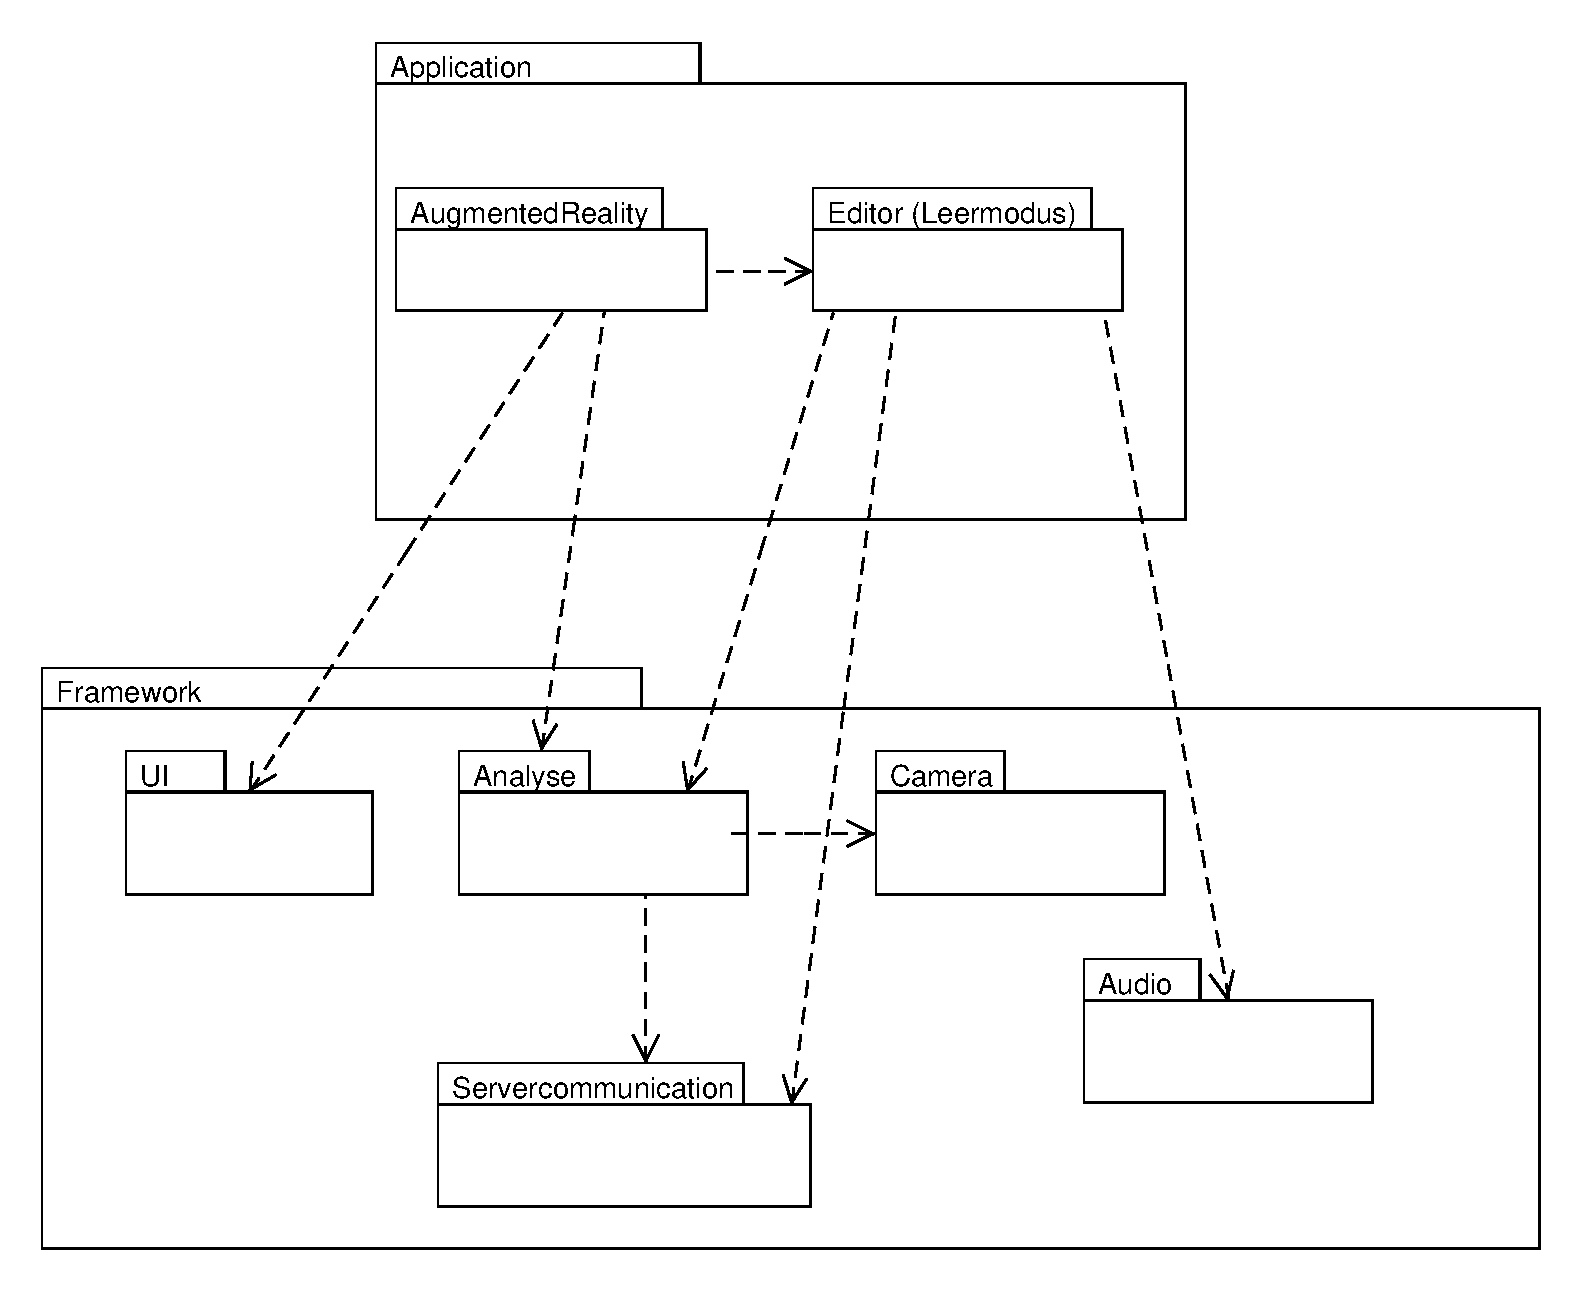
\includegraphics[width=\textwidth]{package_diagram.pdf}
    \caption{Package diagram}
    \label{graph:graph1}
  \end{center}
\end{figure}
We kozen ervoor om de fotoanalyse en de leermodus in aparte packages te steken. Dit kan handig zijn voor usermanagement: zo kan een verschil gemaakt worden tussen gebruikers die mogen analyseren en editeren, en gebruikers die enkel mogen analyseren. We willen de mogelijkheid voorzien dat sommige gebruikers enkel kunnen analyseren en niet kunnen editeren.
\subsection{Contracten tussen subsystemen}
\subsubsection*{Contract 1}
\begin{longtable}{|l|l|p{4cm}|p{5.5cm}|}
\hline\rowcolor{Gray}
\textbf{Interface} & \textbf{Type}& \textbf{Collaborators} & \textbf{Classes}\\ 
\hline
AnalysisInterface&client-server&Analyse en AugmentedReality & FotoAnalyser en ARApplication \\
\hline
\end{longtable}
\subsubsection*{Contract 2}
\begin{longtable}{|l|l|p{5cm}|p{5cm}|}
\hline\rowcolor{Gray}
\textbf{Interface} & \textbf{Type}& \textbf{Collaborators} & \textbf{Classes}\\ 
\hline
EditorInterface&client-server&Editor en AugmentedReality & InformationEditor en ARApplication \\
\hline
\end{longtable}
\subsubsection*{Contract 3}
\begin{longtable}{|l|l|p{4cm}|p{5.4cm}|}
\hline\rowcolor{Gray}
\textbf{Interface} & \textbf{Type}& \textbf{Collaborators} & \textbf{Classes}\\ 
\hline
ServerEditInterface&client-server&Network en Editor & Network en InformationEditor\\
\hline
\end{longtable}
\subsubsection*{Contract 4}
\begin{longtable}{|l|l|p{4cm}|p{4.7cm}|}
\hline\rowcolor{Gray}
\textbf{Interface} & \textbf{Type}& \textbf{Collaborators} & \textbf{Classes}\\ 
\hline
ServerAnalysisInterface&client-server&Network en Analyse & Network en FotoAnalyser  \\
\hline
\end{longtable}
\subsection*{Interface specificatie voor contract 1}
\begin{lstlisting}
interface AnalysisInterface {
	public OverlayDataObject analyse();
}
\end{lstlisting}
\subsection*{Interface specificatie voor contract 2}
\begin{lstlisting}
interface EditorInterface {
	public void edit();
}
\end{lstlisting}
\subsection*{Interface specificatie voor contract 3}
\begin{lstlisting}
interface ServerEditInterface {
	public void updateObject(OverlayDataObject object);
}
\end{lstlisting}
\subsection*{Interface specificatie voor contract 4}
\begin{lstlisting}
interface ServerAnalysisInterface {
	public OverlayDataObject analyseFoto(Foto foto);
}
\end{lstlisting}
\section{Gedetailleerd ontwerp}
\subsection{Analyse}
\subsubsection*{UML klassendiagram:}
\begin{figure}[H]
  \begin{center}
    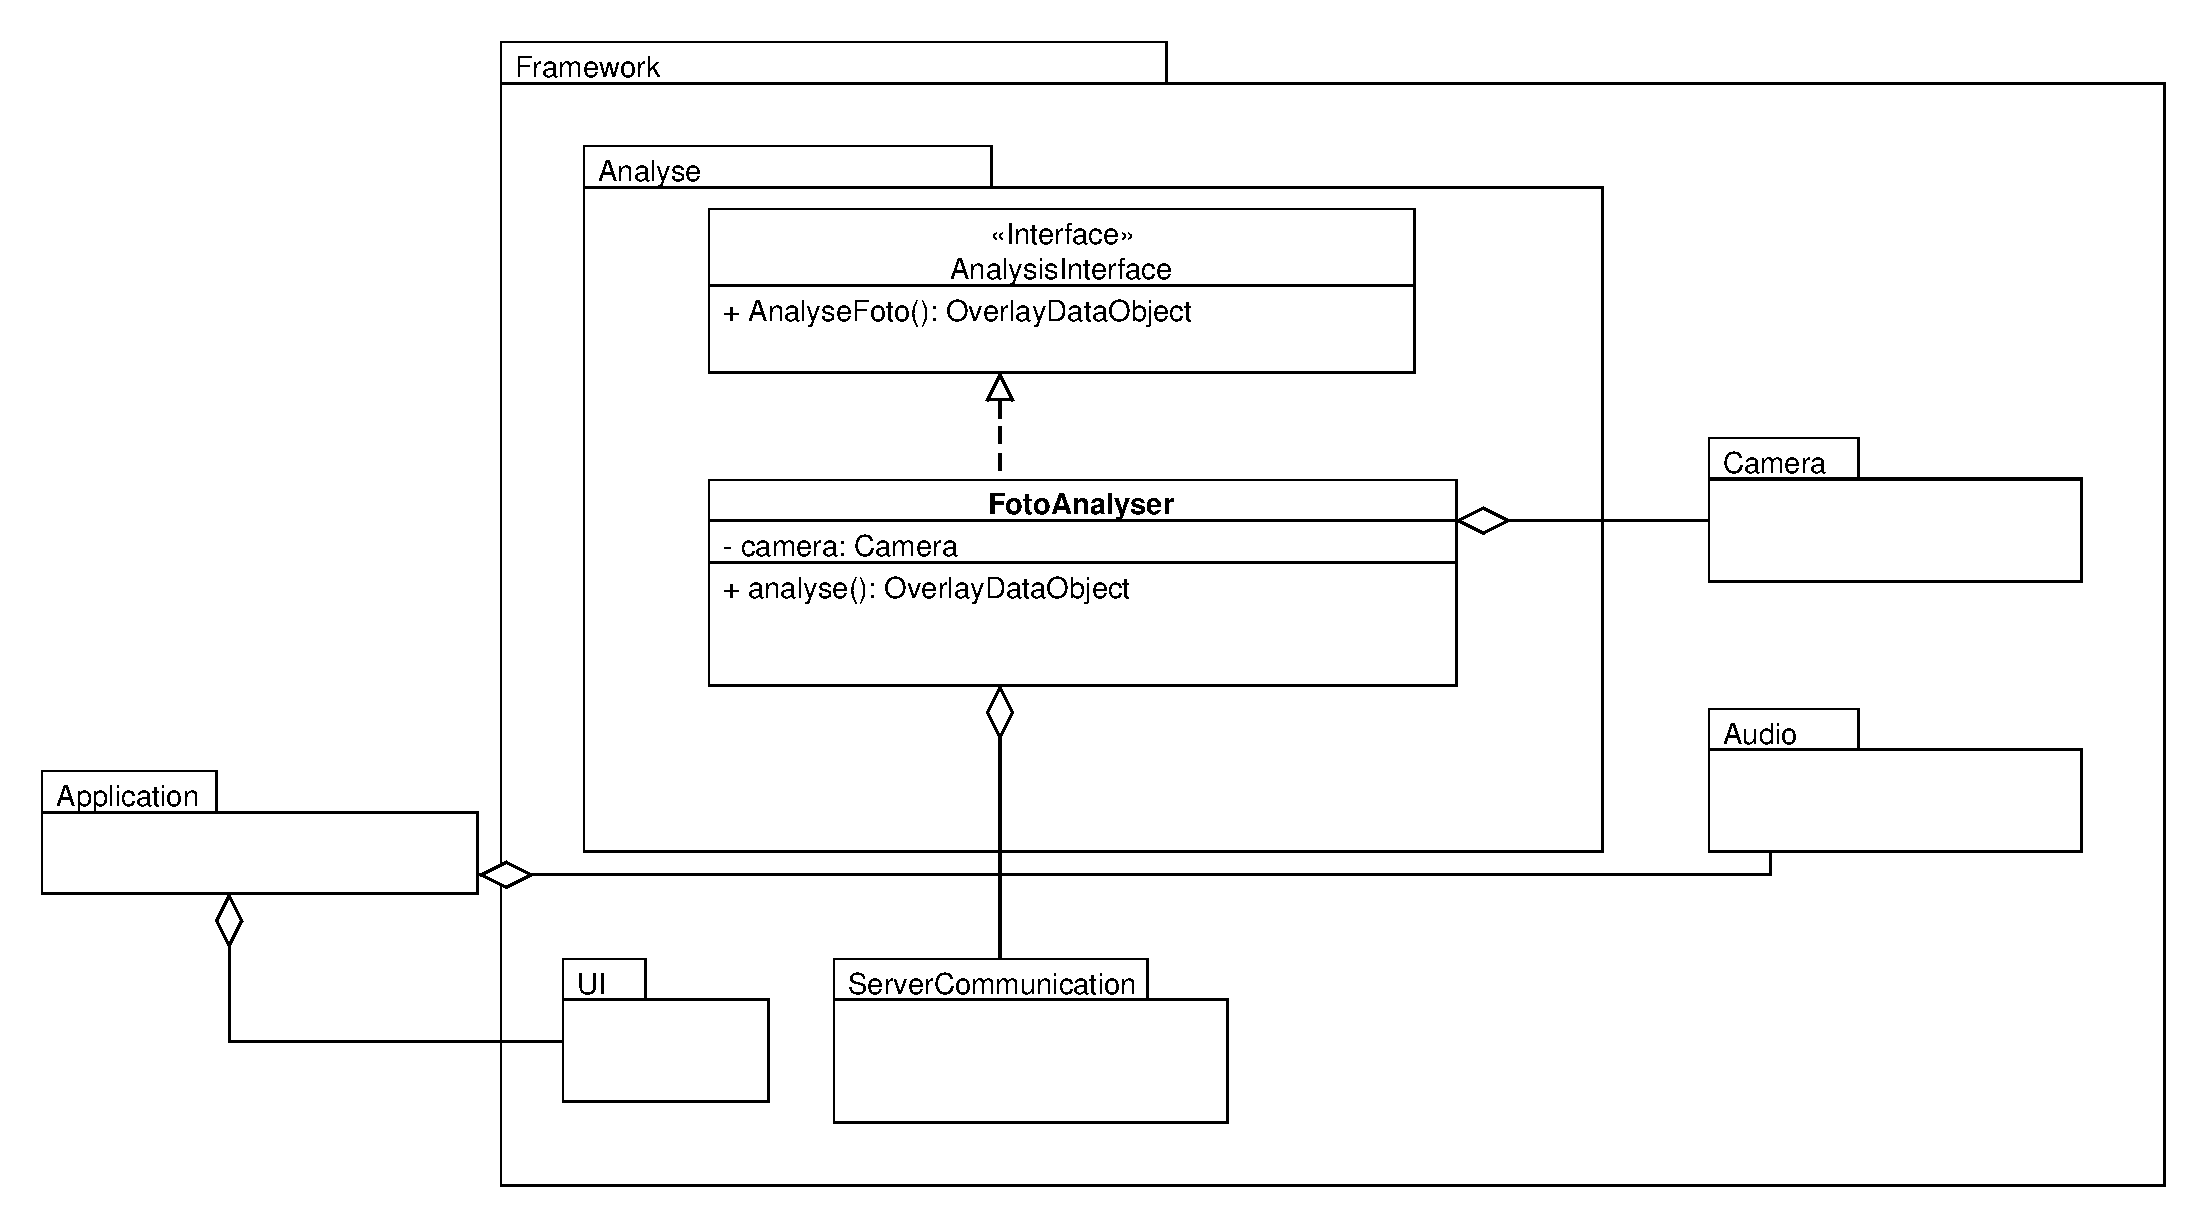
\includegraphics[scale=0.45]{Analyse.pdf}
    \caption{Analyse klassendiagram}
    \label{graph:graph2}
  \end{center}
\end{figure}
\subsubsection*{Algoritmen en datastructuren:}

Datastructuren: \\
De fotoanalyse gebeurt op de server vanwege de performantie. De communicatieklasse tussen de bril en de server zit in het framework zodat andere applicaties hier ook gebruik van kunnen maken.
\begin{itemize}
\item \verb$<FotoAnalyser>$: We nemen een foto en sturen die door naar de server. Voor de fotoherkenning wordt gebruik gemaakt van de scale-invariant feature transform (SIFT) methode. Indien een match gevonden wordt krijgen we een OverlayDataObject terug. Dit object bevat alle informatie over een bepaald object en kan onmiddellijk doorgestuurd worden naar de userinterface. 
\end{itemize}
Verwachte problemen:
\begin{itemize}
\item Het algoritme vindt geen match. Dit kan bijvoorbeeld zijn door de kwaliteit van de foto (bvb. slechte weersomstandigheden, bewegen tijdens het nemen van de foto,...). Hier wordt dan een algoritme op los gelaten dat de kwaliteit van de foto onderzoekt. Is de kwaliteit goed genoeg, kan men ervan uitgaan dat de locatie nog niet in de databank zit en kan de gebruiker worden gevraagd om een nieuwe plaats toe te voegen. Is de foto van een lage kwaliteit, dan zal het algoritme de foto proberen verscherpen en opnieuw proberen te matchen. Wanneer dit faalt, wordt er gemeld aan de gebruiker dat de foto niet geschikt was, en kan deze desgewenst opnieuw proberen.
\end{itemize}
\subsection{Servercommunicatie}
\subsubsection*{UML klassendiagram:}
\begin{figure}[H]
  \begin{center}
    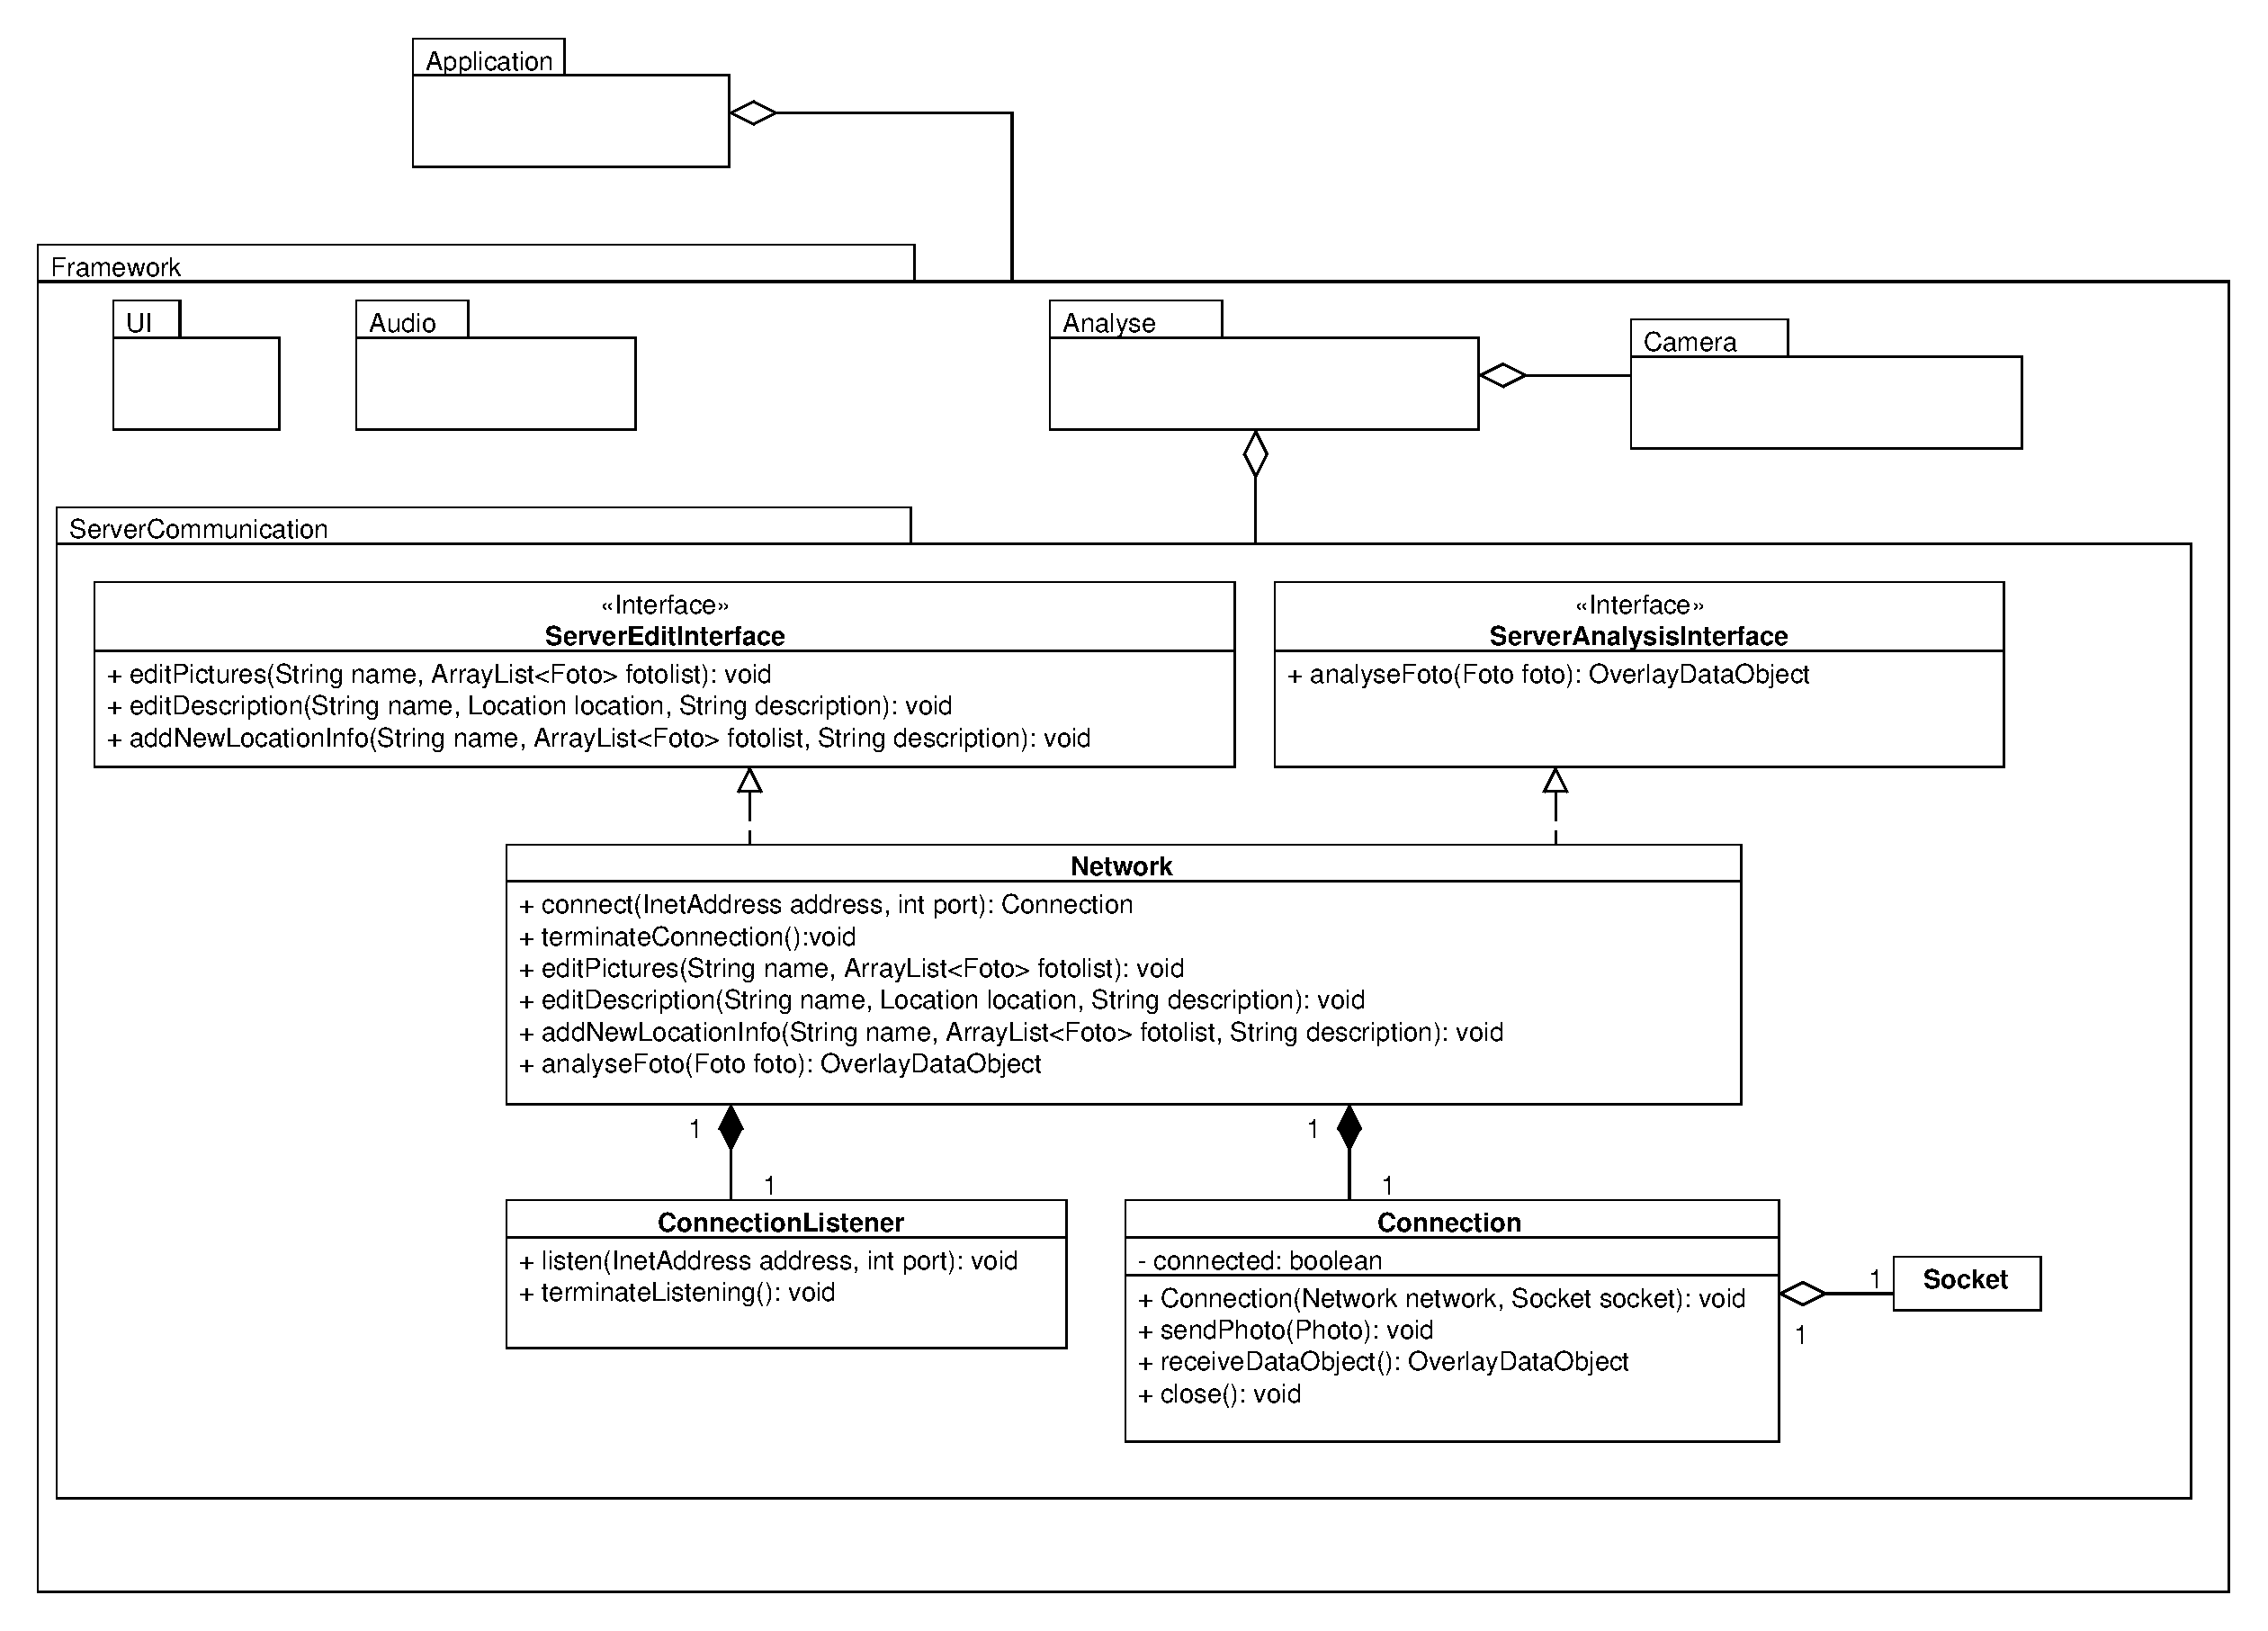
\includegraphics[scale=0.4]{Servercommunicatie.pdf}
    \caption{Servercommunicatie klassendiagram}
    \label{graph:graph3}
  \end{center}
\end{figure}
\subsubsection*{Algoritmen en datastructuren:}
De methoden in de 2 interfaces worden ge\"implementeerd door Network. Zo kunnen de FotoAnalyse en de InformationEditor hier gebruik van maken.
Foto's kunnen aangepast/toegevoegd worden met de methode \verb$editPictures$. In een foto zit ook telkens een locatie als veld.
Een beschrijving kan toegevoegd/aangepast worden zonder een nieuwe foto mee te geven.
Ten slotte kan men ook een nieuw informatiepunt toevoegen in de database.
\par 
Verwachte problemen:
\begin{itemize}
\item Connectie met de server faalt of valt weg.
\end{itemize}
\subsection{Leermodus}
\subsubsection*{UML klassendiagram:}
\begin{figure}[H]
  \begin{center}
    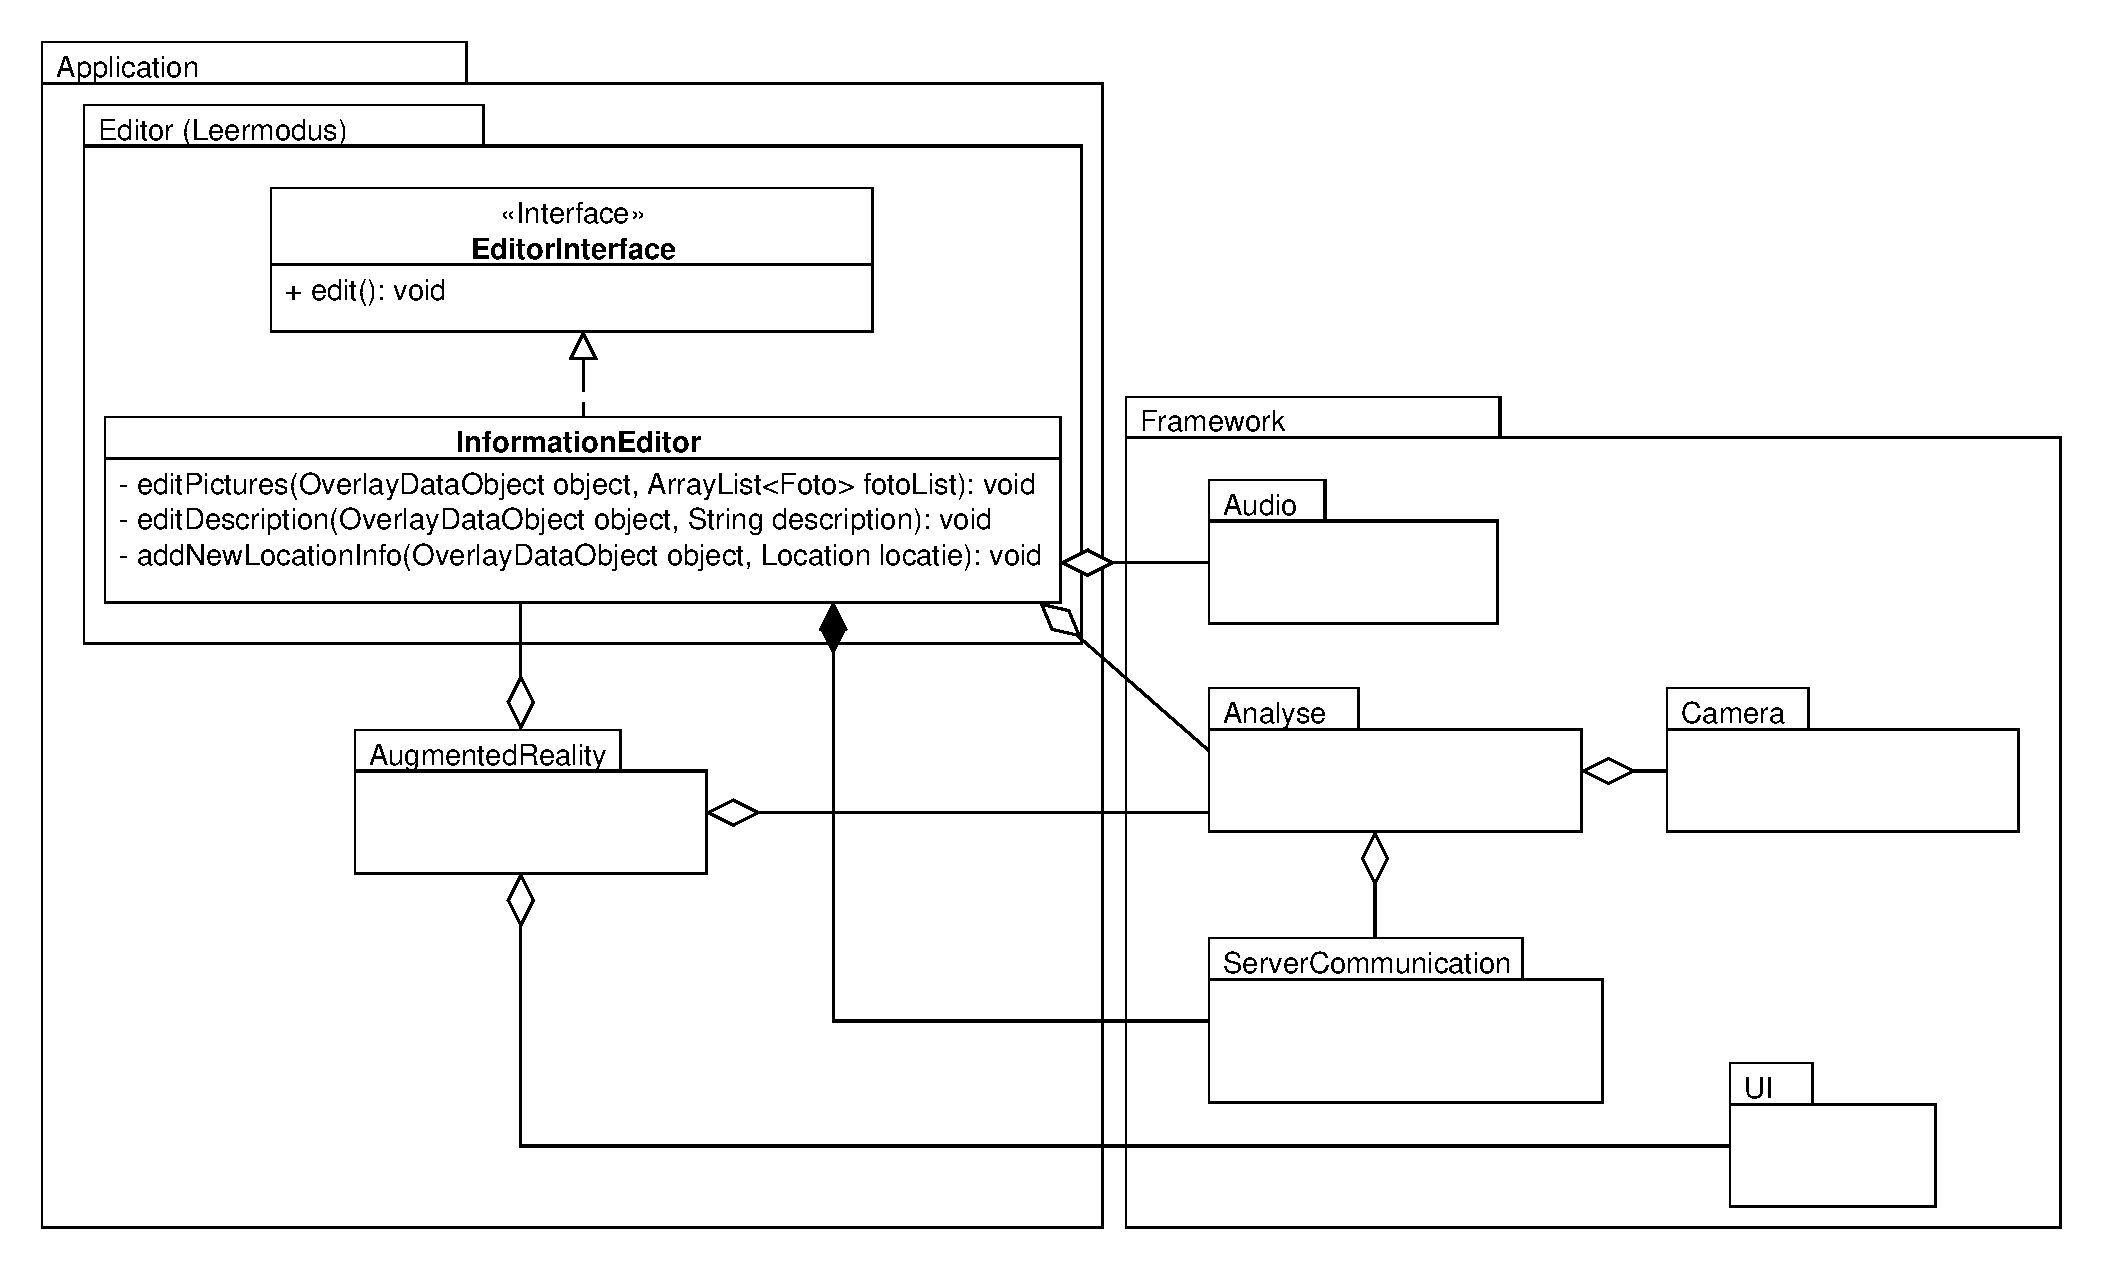
\includegraphics[scale=0.5]{Leermodus.pdf}
    \caption{Leermodus klassendiagram}
    \label{graph:graph2}
  \end{center}
\end{figure}
\subsubsection*{Algoritmen en datastructuren:}
In de leermodus kan de gebruiker info aanpassen/toevoegen met behulp van stemcommando's.\\
\subsection{AugmentedReality}
\subsubsection*{UML klassendiagram:}
\begin{figure}[H]
  \begin{center}
    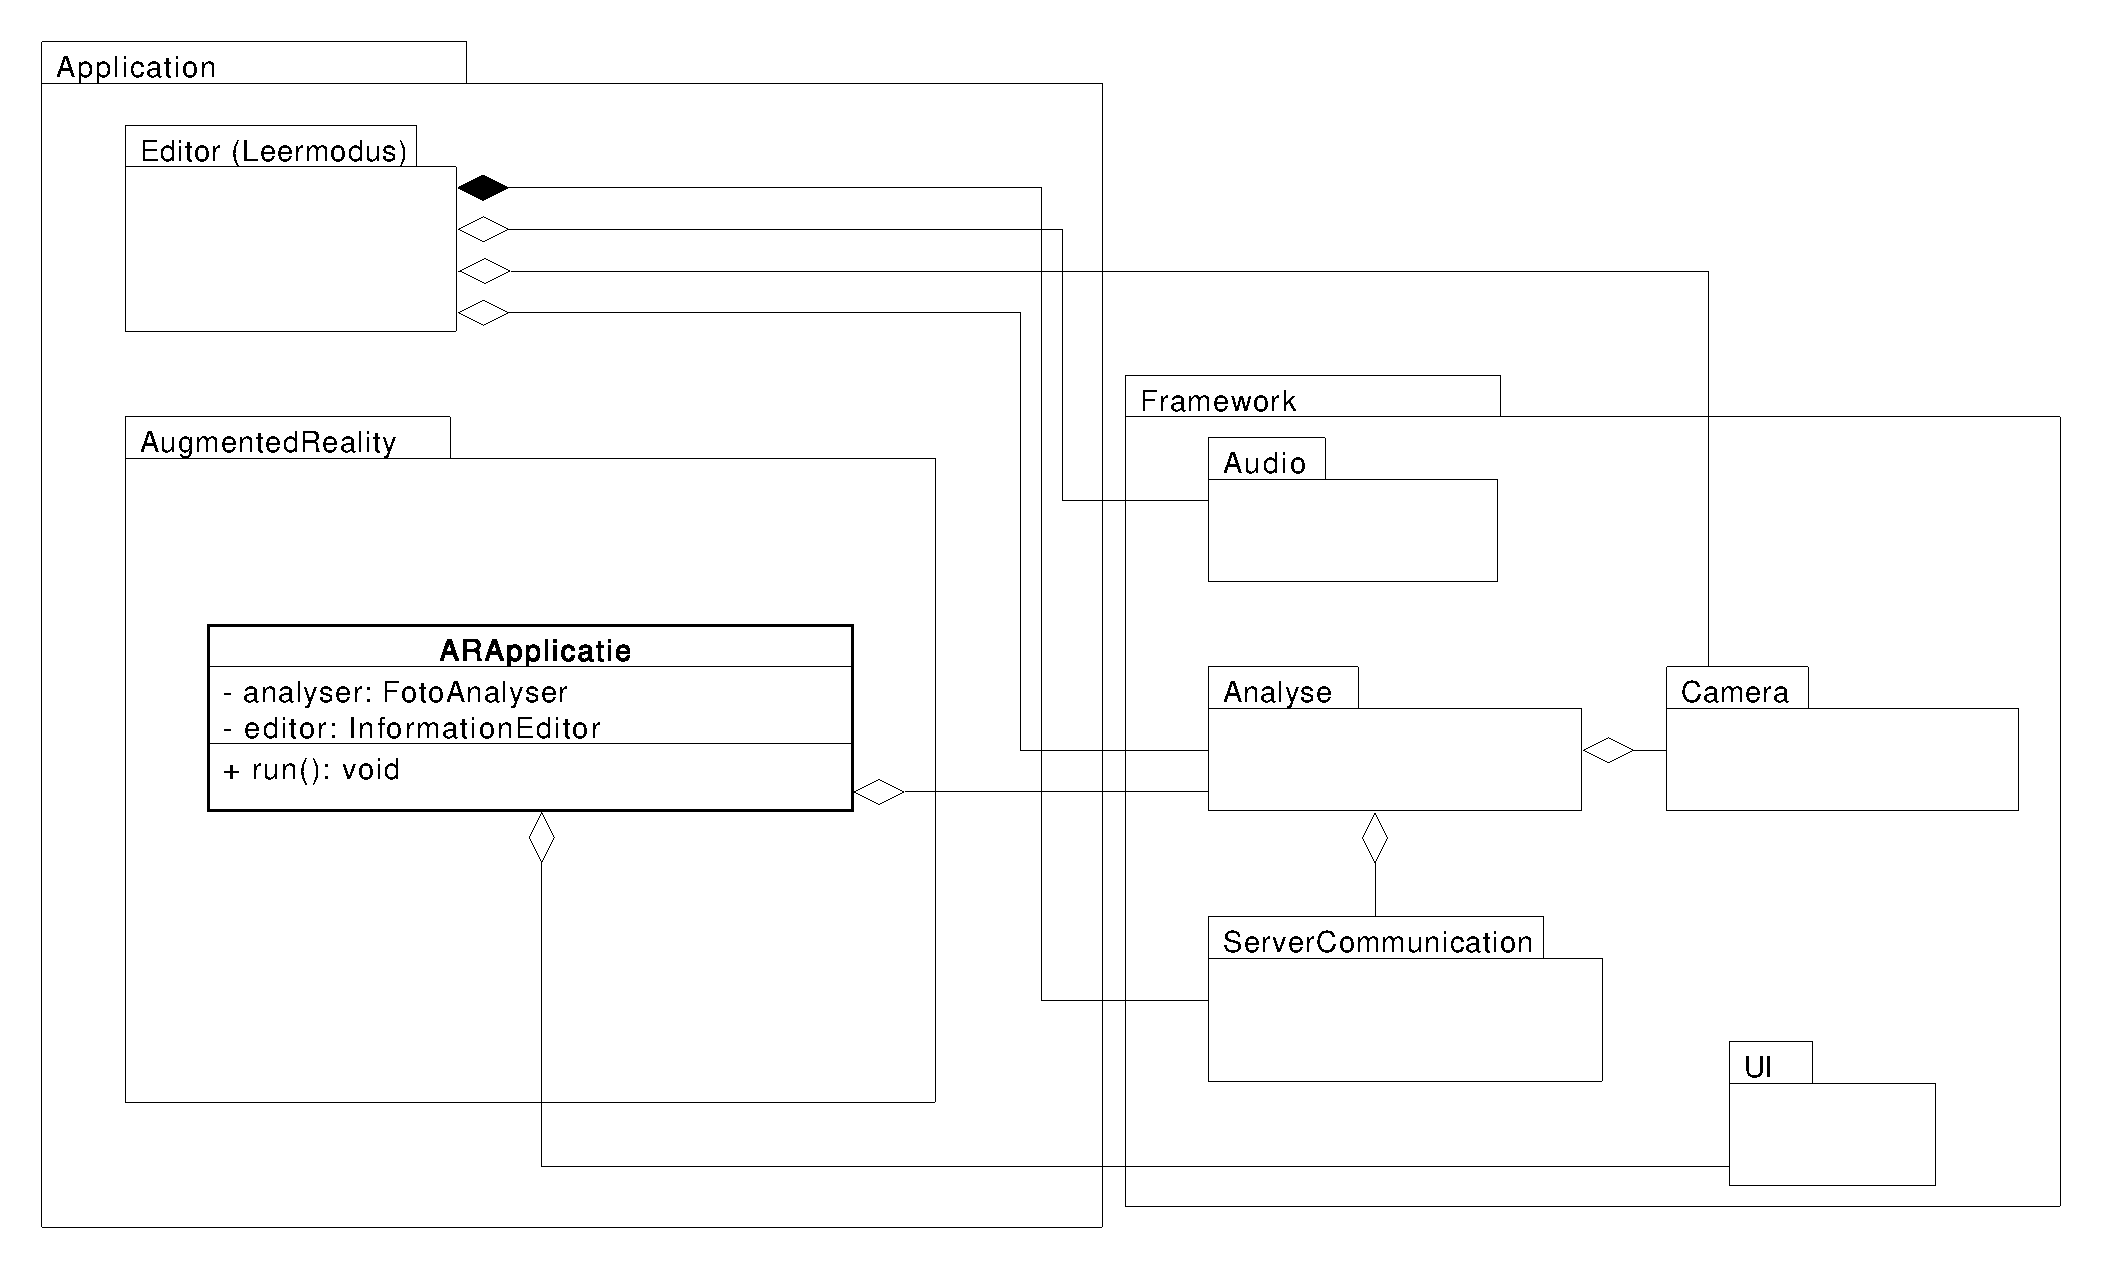
\includegraphics[scale=0.4]{AugmentedReality.pdf}
    \caption{AugmentedReality klassendiagram}
    \label{graph:graph2}
  \end{center}
\end{figure}
\subsubsection*{Algoritmen en datastructuren:}
De ARApplicatie wordt opgestart als de gebruiker hiervoor opdracht geeft in de UI.
\subsection{Audio}
\subsubsection*{UML klassendiagram:}
\begin{figure}[H]
  \begin{center}
    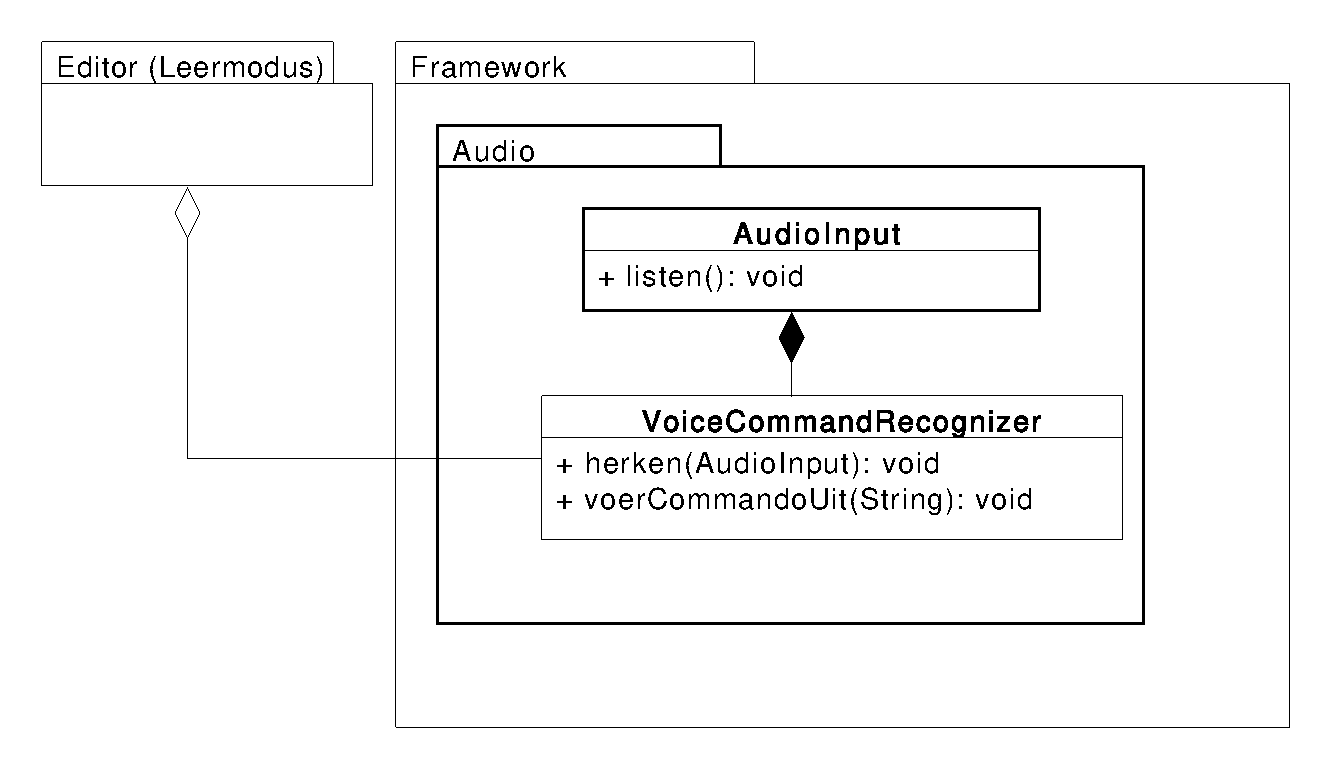
\includegraphics[scale=0.4]{Audio.pdf}
    \caption{AugmentedReality klassendiagram}
    \label{graph:graph2}
  \end{center}
\end{figure}
\subsubsection*{Algoritmen en datastructuren:}
De ARApplicatie wordt opgestart als de gebruiker hiervoor opdracht geeft in de UI.
\end{document}